\subsection{UMAC}\label{sec:umac}
\selectlanguage{russian}

Конструкция UMAC, предложеная в 1999 году (\cite{Black:Halevi:Krawczyk:etc:1999}), также использует подход с быстрым универсальным хэшированием большого исходного сообщения и хэшированием небольшого блока информации надёжной (на 1999 год), но медленной ключевой функцией HMAC-SHA1. В 2003 году вошёл в список алгоримтов, отобранных инициативой NESSIE (\langen{New European Schemes for Signatures, Integrity, and Encryptions}) как безопасный алгоритм вычисления имитовставки. Был стандартизован как RFC 4418 (\cite{rfc4418}). На сегодняшний день не считается криптографически стойким из-за уязвимостей, найденных в SHA-1.

Класс универсальных хэш-функций $\textrm{NH}_K (m)$ описывается следующим образом. Битовая строка $m$ длиной до 1024 32-битовых <<слов>> и размером, кратная 2 <<словам>>, разбивается на отдельные блоки по 32 бита $m_1, m_2, \dots, m_l$. 32-битные ключи $K_1, K_2, \dots, K_l$ получены из исходного ключа $K$ с помощью генератора псевдослучайных чисел. Далее вычисление 64-битового хэша выглядит так: \[\begin{array}{ll}
    \textrm{NH}_K (m) = & ( m_1 +_{32}K_1) \times_{64} (m_2 +_{32} K_2) +_{64} \dots \\
                        & \dots ~ +_{64} ~ \dots \\
                        & \dots ~ +_{64} ~ (m_{l-1} +_{32} K_{l-1}) \times_{64} (m_l+_{32}K_l),
\end{array} \] где $+_{32}$ -- сложение 32-битных строк, в результате которого получается 32-битная сумма, $\times_{64}$ -- произведение двух 32-битных строк, и получаемый 64-битный результат умножения (рис.~\ref{fig:UMAC}).

\begin{figure}
    \centering
    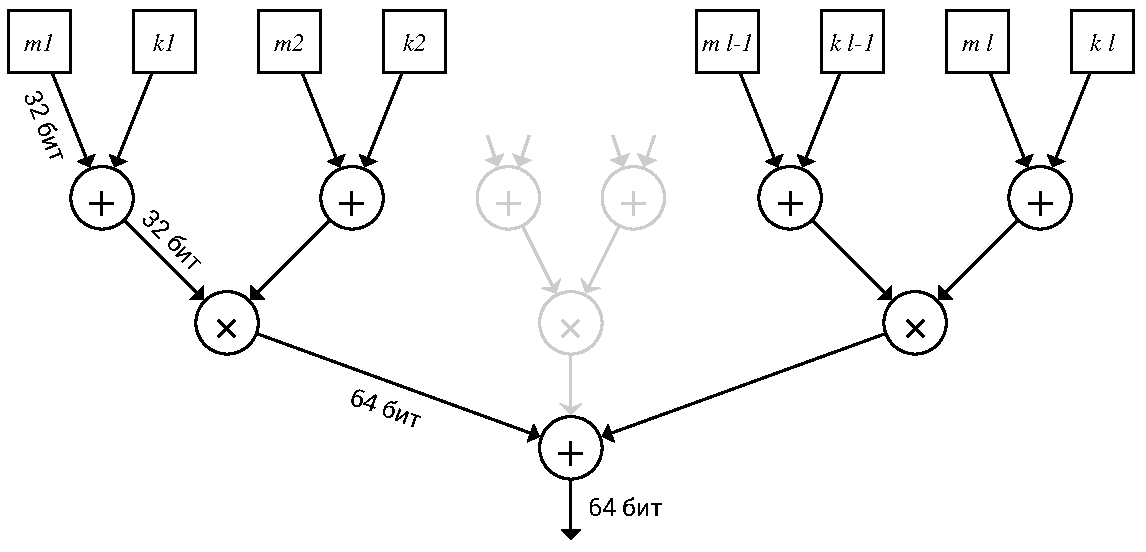
\includegraphics[width=1\textwidth]{pic/UMAC}
    \caption{Универсальне хэширование $\textrm{NH}_K (m)$ в UMAC}
    \label{fig:UMAC}
\end{figure}

Генерация имитовставки делается следующим образом. Предполагается, что вместе с сообщением $m$ передаётся случайная строка \emph{nonce} (должна быть уникальна для каждого сообщения), а у отправителя и получателя есть общий секретный ключ $K$.

\begin{enumerate}
    \item Пусть Len это остаток от деления длины сообщения в битах $|m|$ на 4096:\[
        \textrm{Len} = |m| \bmod 4096.
    \]
    \item Сообщение $m$ в битовом представлении дополняется нулями таким образом, чтобы длина сообщения $|m|$ была кратна 64 бит (8 байт).
    \item Сообщение $m$ разбивается на блоки по 32768 бита (1024 <<слова>> по 32 бита) $m_1, m_2, \dots, m_t$. Последний блок будет содержать от 2 до 1024 <<слов>>.
    \item Каждый блок хэшируется ключевой хэш-функцией $\textrm{NH}_K$, результаты конкатенируются между собой и $Len$:\[
        H_K(m) = \textrm{NH}_K (m_1) ~ \| ~ \textrm{NH}_K (m_2) ~ \| ~ \dots ~ \| ~ \textrm{NH}_K (m_t) ~ \| ~ \textrm{Len}.
    \]
    \item Итоговое значение имитовставки получается через хэширование ключевой функцией HMAC-SHA1:\[
        \textrm{UMAC}_K( m, \textrm{nonce} ) = \textrm{HMAC-SHA1}_K( \textrm{nonce} ~ \| ~ H_K(m) ).
    \]
\end{enumerate}
